% Revised 2026-10-12. One article body is shared by PDF and editable Word.
% Historical source/PDF/Word are preserved in ../history/.
\documentclass[12pt,a4paper]{article}
\usepackage{geometry}
\geometry{top=2.5cm,bottom=2.5cm,left=3cm,right=2cm}
\usepackage{fontspec}
\setmainfont{PT Serif}
\newfontfamily\cyrillicfonttt{DejaVu Sans Mono}
\usepackage{polyglossia}
\setmainlanguage{russian}
\setotherlanguage[variant=american]{english}
\addto\captionsrussian{\renewcommand{\figurename}{Рисунок}\renewcommand{\tablename}{Таблица}}
\usepackage{amsmath,amssymb}
\usepackage{graphicx,array,caption,indentfirst}
\usepackage{titlesec}
\titleformat{\section}{\normalfont\bfseries}{}{0pt}{}
\titlespacing*{\section}{0pt}{14pt}{6pt}
\captionsetup[figure]{labelsep=period,justification=centering,font=small}
\captionsetup[table]{labelsep=period,font={small,bf},justification=raggedright}
\setlength{\parindent}{1.25cm}
\linespread{1.10}
\usepackage[backend=biber,style=gost-numeric,sorting=none]{biblatex}
\addbibresource{../../bibliography/library.bib}
\usepackage[hidelinks]{hyperref}
\setlength{\emergencystretch}{2em}
\clubpenalty=10000
\widowpenalty=10000
\displaywidowpenalty=10000
\renewcommand{\topfraction}{.9}
\renewcommand{\bottomfraction}{.8}
\renewcommand{\textfraction}{.08}
\renewcommand{\floatpagefraction}{.85}
\begin{document}
\renewcommand{\figurename}{Рисунок}
\renewcommand{\tablename}{Таблица}
\noindent УДК 519.872

\bigskip
\noindent Р.С.~Хабаров, к.т.н.\par
\noindent В.А.~Лохвицкий, д.т.н.

\begin{center}
{\large\bfseries СВОЕВРЕМЕННОЕ НАЧАЛО ПАКЕТНОГО ОБСЛУЖИВАНИЯ ПРИ НЕТЕРПЕНИИ ЗАЯВОК: МАРКОВСКОЕ ПРЕДСТАВЛЕНИЕ И ОЦЕНКА ПОГРЕШНОСТИ ЛОКАЛЬНОГО УСЕЧЕНИЯ}
\end{center}

\noindent\textbf{Аннотация.}
Рассматривается одноканальная система массового обслуживания с простейшим входящим потоком, пороговым формированием пакетов и нетерпеливыми заявками. Время обслуживания имеет распределение фазового типа с параметрами, зависящими от размера пакета; времена терпения заявок независимы и распределены экспоненциально. Ожидание меченой заявки описано цепью Маркова с непрерывным временем и поглощением при начале обслуживания или уходе из очереди. По этой цепи рассчитываются вероятности своевременного и позднего начала обслуживания, а также ухода без обслуживания. При фиксированном начальном распределении получена локальная оценка погрешности усечения по числу заявок позади меченой. В исследованной серии с эрланговским и гиперэкспоненциальным обслуживанием уменьшение среднего ожидания среди заявок, начавших обслуживание, сопровождалось снижением вероятности своевременного начала обслуживания для произвольной поступившей заявки. Выявлены случаи ошибочного выбора максимального размера пакета при аппроксимации распределения ожидания по двум моментам. Учёт вероятности нулевого ожидания уменьшил общее число ошибок выбора в рассмотренных расчётах, но увеличил число ошибочных признаний параметров допустимыми.

\medskip
\noindent\textbf{Ключевые слова:} теория массового обслуживания, пакетное обслуживание, нетерпеливые заявки, меченая заявка, порог запуска, фазовое распределение, предельное время ожидания, усечение пространства состояний.

\begin{center}
\textbf{TIMELY START OF BATCH SERVICE WITH CUSTOMER ABANDONMENT: A MARKOV REPRESENTATION AND A LOCAL TRUNCATION ERROR BOUND}

R.S.~Khabarov, V.A.~Lokhvitsky
\end{center}

\begin{otherlanguage}{english}
\noindent\textbf{Abstract.}
We consider a single-server queue with Poisson arrivals, threshold-based batch formation and customer abandonment. Service times have batch-size-dependent phase-type distributions, and customer patience times are independent and exponentially distributed. The waiting process of a tagged customer is described by a continuous-time Markov chain with absorption at service start or abandonment. This chain yields the probabilities of timely service start, late service start and abandonment before service. For a fixed initial distribution, a local error bound is obtained for truncation by the number of customers behind the tagged customer. In the numerical experiments with Erlang and hyperexponential service, a reduction in mean waiting time among customers who entered service accompanied a decrease in the probability of timely service start among all arrivals. Cases of incorrect batch-cap selection are identified for two-moment approximations of the waiting-time distribution. Preserving the zero-wait probability reduces the total number of selection errors in the experiments considered but increases false acceptance of infeasible parameter choices.

\medskip
\noindent\textbf{Keywords:} bulk service, abandonment, tagged customer, dispatch threshold, phase-type distribution, deadline, state-space truncation.
\end{otherlanguage}

\section*{Введение}

При пакетном обслуживании затраты на подготовку одной операции распределяются между несколькими заявками. Выигрыш от совместной обработки сопровождается ожиданием накопления пакета и освобождения канала. Если заявки нетерпеливы, среднее ожидание среди начавших обслуживание характеризует только часть поступивших заявок. При выборе порога запуска и максимального размера пакета поэтому следует учитывать три исхода: начало обслуживания в установленный срок, начало обслуживания после этого срока и уход без обслуживания.

Модели пакетного обслуживания восходят к работе Bailey~\cite{bailey1954}; общее пороговое правило предложено Neuts~\cite{neuts1967}. Распределение времени ожидания при простейшем входящем потоке и экспоненциальном обслуживании по правилу $(a,b)$ исследовано Medhi~\cite{medhi1975}. Основные близкие к рассматриваемой задаче результаты и различия постановок приведены в таблице~\ref{tab:prior}.

\begin{table}[htbp]
\centering\small
\caption{Известные результаты по близким моделям пакетного обслуживания}\label{tab:prior}
\begin{tabular}{p{.22\linewidth}p{.36\linewidth}p{.34\linewidth}}
\hline
Работа & Рассмотренный результат & Существенное отличие \\\hline
Medhi~\cite{medhi1975} & Стационарное распределение времени ожидания и его моменты при правиле $(a,b)$ & Простейший поток, экспоненциальное обслуживание; нетерпение не учитывается \\
Banerjee и др.~\cite{banerjee2015} & Совместные стационарные распределения при марковском входящем потоке и зависимости обслуживания от размера пакета & Ограниченная вместимость очереди; более общий входящий поток \\
Claeys и др.~\cite{claeys2013} & Аппроксимация дополнительной функции распределения времени ожидания по полюсам и вычетам & Дискретное время, групповой входящий поток, ограничение времени накопления \\
van Ommeren и др.~\cite{vanommer2020} & Фазовое представление времени ожидания с учётом числа заявок перед меченой и позади неё & Неоднородные каналы; интенсивность обслуживания не зависит от размера пакета; нетерпение не учитывается \\
Chaudhry и др.~\cite{chaudhry2023} & Расчёт распределения длины очереди методом корней и распределения времени ожидания с аппроксимацией Паде & Ограниченная вместимость очереди, одинаковый закон обслуживания пакетов \\
\hline
\end{tabular}
\end{table}

Цель работы --- построить расчётную схему для выбора порога запуска и максимального размера пакета по вероятности своевременного начала обслуживания с учётом ухода заявок из очереди. Ожидание представляется временем до поглощения; состояние включает числа заявок перед меченой заявкой и позади неё. Такой способ описания пороговой пакетной системы использован в работе~\cite{vanommer2020}. В настоящей работе он применяется к обслуживанию, зависящему от размера пакета, и экспоненциальному терпению с уходом всех ожидающих заявок. Для усечения числа заявок позади меченой получена оценка погрешности при фиксированном начальном распределении. В численных примерах сопоставлены требования к своевременности для начавших обслуживание и для всех поступивших заявок, а также решения о выборе размера пакета по марковской модели и аппроксимациям распределения ожидания.

Одной из областей применения пакетного обслуживания является обработка запросов к большим языковым моделям (БЯМ; англ. large language models, LLM)~\cite{yu2022orca}. Зависимость длительности обработки от размера пакета учитывается в моделях нейросетевых инференс-серверов~\cite{inoue2021}. Применительно к БЯМ рассматриваемая модель описывает отдельную операцию с неизменным составом пакета; предельный срок относится к началу этой операции, а не к завершению всего запроса.

\section*{Постановка задачи и показатели своевременности обслуживания}

Рассмотрим одноканальную систему с простейшим (однородным пуассоновским) входящим потоком интенсивности $\lambda>0$ и неограниченной очередью. Заявки выбираются на обслуживание в порядке поступления (дисциплина FIFO). При свободном канале обслуживание начинается, если в очереди находится не менее $a$ заявок. Из $j$ ожидающих в пакет включаются первые $\min(b,j)$ заявок, где $1\leq a\leq b$. Порог $a$ задаёт условие начала обслуживания, а $b$ --- максимальный размер пакета. Состав пакета во время обслуживания не изменяется; все его заявки одновременно завершают обслуживание через случайное время $S_i$, закон которого зависит от размера пакета $i$.

Для времени $S_i$ используем распределение фазового типа с представлением $(\beta_i,T_i)$, где $\beta_i$ --- вектор начальных вероятностей, $T_i$ --- подгенератор переходов между фазами. Начальные вероятности неотрицательны и в сумме равны единице; завершение обслуживания соответствует поглощению, наступающему с вероятностью единица. Такое представление позволяет учитывать неэкспоненциальное обслуживание. Далее рассматриваются распределения Эрланга $E_k$ с коэффициентом вариации $1/\sqrt{k}$ и гиперэкспоненциальное $H_2$ с коэффициентом вариации не меньше единицы.

Время терпения отсчитывается от поступления заявки и имеет экспоненциальное распределение $A\sim\operatorname{Exp}(\gamma)$ при $\gamma>0$. Заявка уходит, если её терпение истекло до начала обслуживания; после начала обслуживания уход не допускается. Случай $\gamma=0$ соответствует отсутствию уходов. Времена терпения разных заявок независимы между собой и от входящего потока. При формировании каждого пакета его время обслуживания выбирается по закону, соответствующему размеру пакета, независимо от предшествующей истории, будущих поступлений и времён терпения.

Выберем поступившую в стационарную систему заявку и назовём её меченой. Обозначим через $S$ событие начала её обслуживания, через $A_b$ --- уход без обслуживания, а через $W$ --- время от поступления до начала обслуживания, определённое на событии $S$. Пусть $D\geq0$ --- установленное предельное время ожидания. Введём вероятности
\begin{align}
 p_S&=P(S), & p_A&=P(A_b),\\
 L(D)&=P(S,W>D), & S(D)&=P(S,W\leq D).
\end{align}
Три безусловные вероятности удовлетворяют $S(D)+L(D)+p_A=1$.
При $p_S>0$ дополнительная функция распределения (ДФР) времени ожидания при условии начала обслуживания и вероятность того, что поступившая заявка не начнёт обслуживание в срок, связаны соотношением
\begin{equation}\label{eq:sla}
 \overline F_S(D)=\frac{L(D)}{p_S},\qquad
 1-S(D)=p_A+p_S\overline F_S(D).
\end{equation}
Таким образом, условный критерий $\overline F_S(D)\leq\varepsilon$ ограничивает долю превысивших срок среди заявок, начавших обслуживание. Безусловный критерий $1-S(D)\leq\varepsilon$ ограничивает долю всех поступивших заявок, для которых своевременное начало обслуживания не состоялось: они либо начали обслуживание позднее $D$, либо ушли из очереди. При включении требования в соглашение об уровне обслуживания (SLA) необходимо указать, к какой совокупности заявок оно относится. Полное время пребывания до завершения обслуживания обозначим $V$; предельный срок $D$ в настоящей работе ограничивает ожидание.

Под устойчивостью далее понимается положительная возвратность цепи состояний системы на её достижимом неприводимом классе. В отсутствие нетерпения при конечном $b$ условие устойчивости имеет вид $\lambda E[S_b]<b$: при достаточно большой очереди обслуживаются полные пакеты размера $b$. При $\gamma>0$, конечном числе фаз и конечных положительных интенсивностях обслуживания уход ожидающих заявок обеспечивает отрицательный снос числа заявок вне конечного множества состояний. Средняя скорость изменения числа заявок в системе не превосходит $\lambda-\gamma j$, где $j$ --- число ожидающих заявок; число обслуживаемых ограничено величиной $b$. Поэтому $\lambda E[S_b]/b$ используется как характеристика нагрузки, а фактическая доля времени занятости канала определяется отдельно.

\section*{Марковское представление и расчёт показателей ожидания}

При занятом канале состояние системы задаётся тройкой $(i,\varphi,j)$, где $i$ --- размер обслуживаемого пакета, $\varphi$ --- текущая фаза обслуживания, $j$ --- число заявок в очереди. Состояние простоя обозначим $I_j$, $0\leq j<a$. Поступление заявки увеличивает $j$ на единицу, а уход из очереди уменьшает его на единицу с суммарной интенсивностью $j\gamma$. Переходы между фазами задаются матрицей $T_i$; интенсивность завершения обслуживания из фазы $\varphi$ равна соответствующей компоненте вектора $\nu_i=-T_i\mathbf1$, где $\mathbf1$ --- столбец единиц. После завершения обслуживания при $j\geq a$ формируется пакет размера $m=\min(b,j)$, начальная фаза выбирается согласно распределению $\beta_m$, а в очереди остаются $j-m$ заявок. При $j<a$ система переходит в состояние $I_j$. Поступление заявки в состоянии $I_{a-1}$ приводит к началу обслуживания пакета размера $a$.

\begin{figure}[htbp]\centering
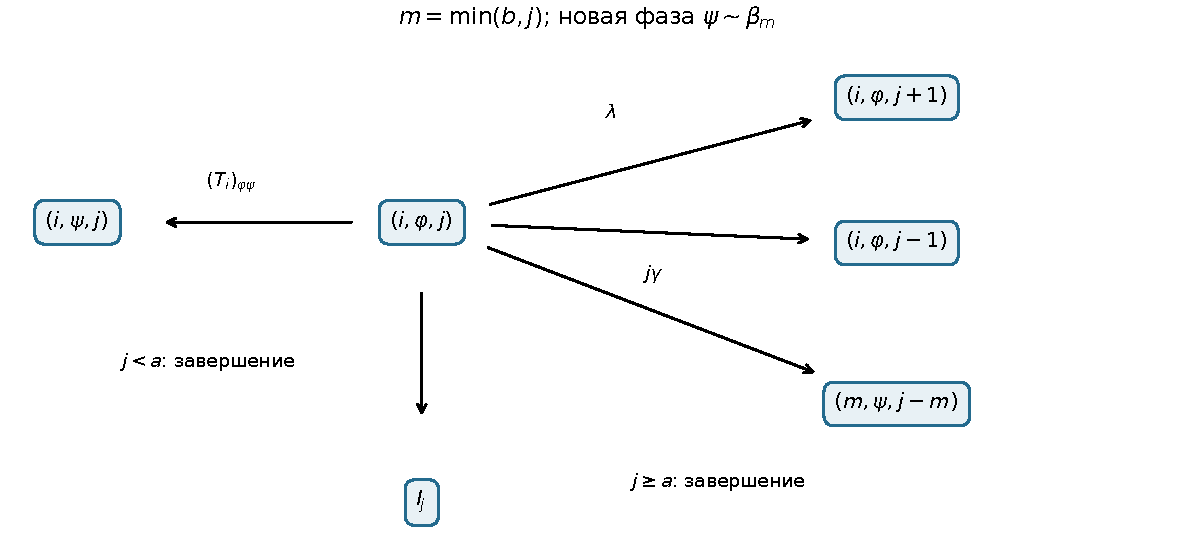
\includegraphics[width=\linewidth]{../figures/revision_queue.pdf}
\caption{Переходы из состояния с занятым каналом. После завершения обслуживания в следующий пакет включаются $m=\min(b,j)$ заявок. Интенсивности соответствующих переходов равны $\nu_{i,\varphi}\beta_{m,\psi}$, а при переходе в простой --- $\nu_{i,\varphi}$.}\label{fig:queue}
\end{figure}

Согласно принципу PASTA (Poisson Arrivals See Time Averages), распределение состояний, наблюдаемых поступающей заявкой, совпадает со стационарным распределением $\pi$. Вероятность немедленного начала обслуживания равна $p_0=\pi(I_{a-1})$: поступившая заявка застаёт свободный канал и $a-1$ ожидающих заявок, дополняя пакет до порога запуска. Среди заявок, начавших обслуживание, доля заявок с нулевым ожиданием равна $P(W=0\mid S)=p_0/p_S$. Поэтому условная функция распределения времени ожидания имеет в нуле скачок этой величины. Точку, в которой сосредоточена положительная вероятность, называют атомом распределения; здесь это атом в нуле.

Остальные стационарные вероятности задают начальное распределение процесса ожидания. Для численного расчёта $\pi$ используется приближение $\pi_N$, получаемое из системы $\pi_N Q_N=0$, $\pi_N\mathbf1=1$. Генератор $Q_N$ строится на состояниях с $j\leq N$ с исключением переходов, соответствующих поступлению заявки при $j=N$.

Проследим за заявкой, не начавшей обслуживание немедленно, от её поступления до начала обслуживания или ухода из очереди. Через $R$ и $K$ обозначим числа заявок, ожидающих соответственно перед ней и позади неё. Если поступившая заявка застала $j$ ожидающих, начальные значения равны $R=j$, $K=0$. Состояние включает также режим канала, а при занятом канале --- размер текущего пакета и фазу обслуживания. Уже обслуживаемые заявки в $R$ и $K$ не входят. Наряду с переходами между фазами и уходом меченой заявки с интенсивностью $\gamma$ учитываются переходы
\begin{equation}
 R\longrightarrow R-1\quad(R\gamma),\qquad
 K\longrightarrow K+1\quad(\lambda),\qquad
 K\longrightarrow K-1\quad(K\gamma),
\end{equation}
Интенсивности указаны в скобках. Переходы при завершении обслуживания пакета показаны на рисунке~\ref{fig:tagged}.

\begin{figure}[htbp]\centering
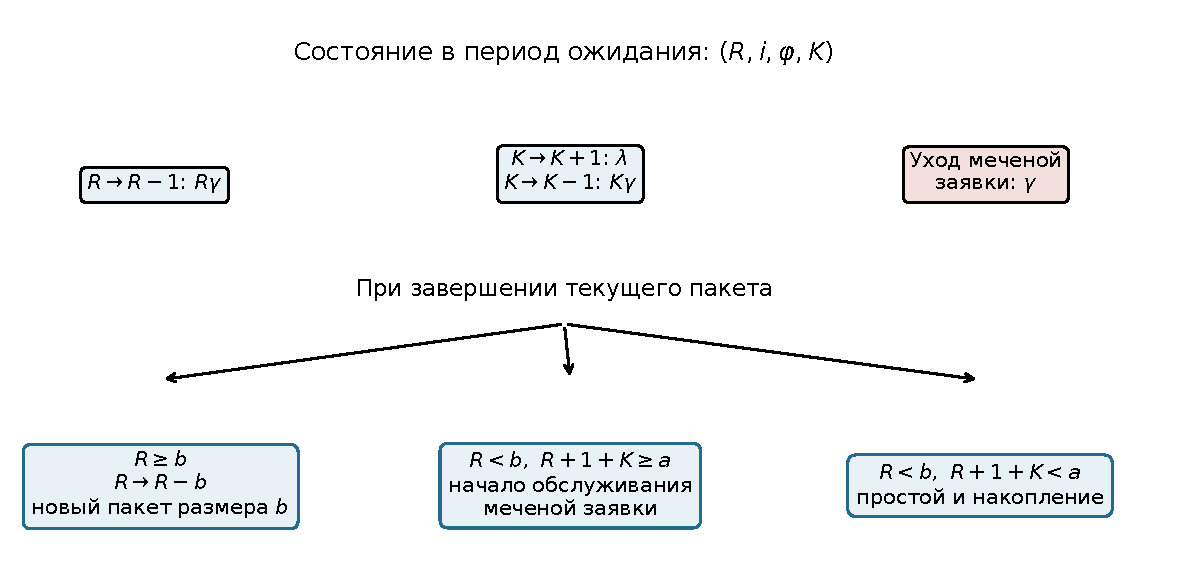
\includegraphics[width=\linewidth]{../figures/revision_tagged.pdf}
\caption{Процесс ожидания меченой заявки: учёт числа заявок перед ней и позади неё. При простое продолжаются поступления и уходы заявок; обслуживание начинается при достижении порога запуска.}\label{fig:tagged}
\end{figure}

Если сформированный после поступления меченой заявки пакет не включает её, его размер равен $b$. Действительно, при меньшем размере пакета все ожидающие заявки, в том числе меченая, должны были бы войти в него в соответствии с дисциплиной FIFO. Следовательно, произвольный размер $i$ имеет только пакет, обслуживаемый в момент поступления меченой заявки. При $R\geq b$ завершение текущего обслуживания приводит к началу обслуживания полного пакета: число $R$ уменьшается на $b$, а начальная фаза выбирается заново согласно $\beta_b$. При $R<b$ меченая заявка поступает на обслуживание тогда и только тогда, когда $R+1+K\geq a$. В противном случае канал простаивает до накопления необходимого числа заявок.

Для численного расчёта ограничим число заявок позади условием $K\leq C$ и выберем конечное множество начальных состояний. Обозначим через $T$ подгенератор на состояниях продолжающегося ожидания, через $s$ --- столбец интенсивностей начала обслуживания, через $\alpha$ --- начальный вектор весов этих состояний, полученный из стационарного распределения. Вероятность немедленного начала обслуживания $p_0$ учитывается отдельно; вектор $\alpha$ не нормируется к единице. Два вида поглощения --- начало обслуживания и уход --- задают равенство $T\mathbf1+s+\gamma\mathbf1=0$. По стандартным формулам для цепи Маркова с поглощением получаем
\begin{align}
 h&=(-T)^{-1}s,& p_S&=p_0+\alpha h,\\
 L(D)&=\alpha e^{TD}h,& p_A&=\gamma\alpha(-T)^{-1}\mathbf1,\label{eq:ph}\\
 E[W^n\mid S]&=\frac{n!\alpha(-T)^{-n-1}s}{p_S},&
 S(D)&=p_S-L(D).
\end{align}
Формула для моментов справедлива при $n\geq1$. В частности, $\overline F_S(0)=1-p_0/p_S$. Эти соотношения точны для конечной цепи и дают приближение для исходной системы с неограниченной очередью. Если исключены начальные состояния суммарной вероятности $\delta$, рассчитанные вероятности удовлетворяют равенству $p_S+p_A=1-\delta$; исключённая вероятность учитывается отдельно от вероятностей исходов.

\section*{Локальная оценка погрешности усечения}

При $a>1$ и $\gamma>0$ число $K$ определяет как возможность накопления пакета, так и интенсивность ухода заявок позади меченой. Для конечного расчёта переходы из $K=C$ в $K=C+1$ исключаются. Погрешность такого усечения оценивается через вероятность достижения границы до истечения времени терпения меченой заявки. При $a=1$ число $K$ не влияет на её ожидание и исключается из описания состояния. При $\gamma=0$ оно не уменьшается, поэтому значения $K\geq a-1$ можно объединить в одно состояние без погрешности.

\noindent\textbf{Утверждение.}
Пусть $a>1$, $\gamma>0$. Вспомогательный процесс $K(t)$ описывается схемой размножения и гибели с интенсивностями $\lambda$ и $k\gamma$, $K(0)=0$. Обозначим через $H_C$ момент первого перехода $C\to C+1$, а через $A\sim\operatorname{Exp}(\gamma)$ --- независимое время терпения меченой заявки. Рассмотрим усечённый процесс, в котором исключены переходы из $C$ в $C+1$, где $C\geq a-1$. При одинаковом начальном состоянии абсолютная погрешность вероятности любого события, определяемого уходом или временем начала обслуживания меченой заявки, не превосходит
\begin{equation}\label{eq:bound}
 B_0(C)=P(H_C<A)=e_0^{\mathsf T}M_C^{-1}\lambda e_C,
\end{equation}
где $e_k$ --- единичный вектор с ненулевой компонентой на месте $k$, а $M_C$ --- трёхдиагональная матрица размера $C+1$ с элементами
\begin{equation}
 (M_C)_{kk}=\lambda+(k+1)\gamma,\quad
 (M_C)_{k,k+1}=-\lambda,\quad (M_C)_{k,k-1}=-k\gamma.
\end{equation}
Для ненормированных моментов $E[W^n\mathbf1_S]$, где $\mathbf1_S$ --- индикатор события $S$, соответствующая оценка погрешности имеет вид
\begin{equation}\label{eq:momentbound}
 B_n(C)=n!\sum_{j=0}^{n}
 \frac{e_0^{\mathsf T}M_C^{-j-1}\lambda e_C}{\gamma^{n-j}}.
\end{equation}

\noindent\textbf{Доказательство.}
До начала обслуживания меченой заявки ни одна из заявок позади неё не может быть включена в пакет в силу дисциплины FIFO. Поэтому процесс $K$ допускает независимое от обслуживания продолжение по схеме размножения и гибели. Исходный и усечённый процессы можно построить на общих поступлениях и уходах так, чтобы их траектории совпадали до момента $H_C$. Различие исходов возможно лишь при $H_C<A$: при $H_C\geq A$ в обоих процессах до возможного расхождения уже произошло одно и то же поглощение --- начало обслуживания или уход меченой заявки. Решение уравнений для вероятности достижения границы при независимом поглощении с интенсивностью $\gamma$ даёт~\eqref{eq:bound}. При различии траекторий оба значения $W^n\mathbf1_S$ заключены между $0$ и $A^n$, поэтому математическое ожидание их абсолютной разности не превосходит $E[A^n;H_C<A]$. После момента $H_C$ остаточное время терпения имеет то же экспоненциальное распределение. Разлагая степень суммы $H_C$ и этого остатка и используя формулу резольвенты для $E[H_C^j e^{-\gamma H_C}]$, получаем~\eqref{eq:momentbound}.\hfill$\square$

Оценки~\eqref{eq:bound}, \eqref{eq:momentbound} равномерны по начальным состояниям с $K=0$ и потому применимы при любом фиксированном начальном распределении. Если при $\gamma>0$ дополнительно исключить начальные состояния суммарной вероятности $\delta$, оценки погрешности вероятностей увеличиваются не более чем на $\delta$, а ненормированных моментов --- на $\delta n!/\gamma^n$. Для условных моментов и условной ДФР требуется также учёт погрешности знаменателя $p_S$. Локальная оценка характеризует усечение процесса ожидания при заданных начальных вероятностях; погрешность замены $\pi$ на $\pi_N$ в неё не входит.

\section*{Численная схема и проверка расчёта}

Число $R$ в процессе ожидания не увеличивается. Поэтому системы линейных уравнений с матрицей $-T$ решаются последовательно по блокам, соответствующим значениям $R$, с повторным использованием матричных разложений. Произведение матричной экспоненты на вектор вычисляется с учётом разреженности матрицы, без построения всех элементов экспоненты. В численных примерах граница $C$ выбирается из условия $B_0(C)\leq10^{-13}$, суммарная вероятность исключаемых начальных состояний не превышает $10^{-13}$, а число состояний цепи ограничено 300\,000. При $\gamma=0$ начальные состояния не исключаются.

Для проверки стационарного расчёта последовательно принимаются $N=200,400,800,1600$. Расчёт принимается при одновременном выполнении двух условий: суммарная вероятность состояний с $j=N$ не превышает $10^{-10}$, а изменения первых двух моментов и рассчитываемых вероятностей при увеличении $N$ не превышают $10^{-7}$. Эти условия служат численным критерием сходимости, а не оценкой полной погрешности. Дополнительно используются балансовые соотношения, аналитический частный случай и независимое имитационное моделирование.

Пусть $L_q$ --- стационарное число ожидающих заявок. Для дополнительной проверки используем равенство интенсивностей ухода, вычисленных двумя способами:
\begin{equation}\label{eq:flow}
 \lambda p_A=\gamma E[L_q].
\end{equation}
При $\gamma=0$ по формуле Литтла среднее время ожидания равно $E[L_q]/\lambda$. В этом случае среднее время обслуживания произвольной заявки определяется с весами по потоку заявок: если $f_i$ --- интенсивность завершения обслуживания пакетов размера $i$, то $E[S_{\mathrm{job}}]=\sum_i i f_i E[S_i]/\lambda$. При наличии нетерпения отношение $E[L_q]/\lambda$ определяет среднее время нахождения в очереди всех поступивших заявок, включая ушедшие, и не совпадает с $E[W\mid S]$.

Аналитический частный случай получается при $a=b=2$, $R=0$, остаточном времени обслуживания с распределением $\operatorname{Exp}(1)$ и $\lambda=\gamma=1$. При $K(0)=0$ число заявок позади до завершения текущего обслуживания имеет распределение $\operatorname{Poi}(1-e^{-t})$. Если обслуживание завершилось при $K=0$, вероятность поступления следующей заявки раньше ухода меченой равна $1/2$. Отсюда
\begin{equation}
 P(S)=\int_0^\infty e^{-2t}\left[1-\tfrac12 e^{-(1-e^{-t})}\right]dt
 =\frac{1-e^{-1}}2,\quad p_A=0{,}6839397206.
\end{equation}
Этот результат используется для проверки переходов, учитывающих поступление и уход заявок позади меченой.

\noindent\textbf{Параметры численных примеров.}
Среднее время обслуживания пакета задано зависимостью $g(i)=0{,}1438i+1{,}8874$, заимствованной из работы~\cite{inoue2021}. Для сравнения законов обслуживания время выражено в условных единицах, а интенсивности $\lambda$ и $\gamma$ --- в обратных единицах времени. Коэффициенты исходной зависимости, полученные Inoue в миллисекундах, используются как параметры расчётного примера, без привязки к конкретному устройству.

Распределение $E_k$ задаётся $k$ последовательными фазами одинаковой интенсивности $k/g(i)$. Для $H_2$ при коэффициенте вариации $c_v\geq1$ вероятность выбора первой ветви равна $p=(1+\sqrt{(c_v^2-1)/(c_v^2+1)})/2$, а интенсивности ветвей --- $2p/g(i)$ и $2(1-p)/g(i)$. Вероятность выбора второй ветви равна $1-p$. При равенстве интенсивностей получается экспоненциальное распределение. В расчётах для $H_2$ принято $c_v=1{,}5$. Начальная фаза каждого нового пакета выбирается независимо от предыдущего обслуживания.

Влияние нетерпения рассматривается на 12 вариантах: законы обслуживания $E_3$ и $H_2$ при $\lambda=0{,}8$, $a=2$, $b=8$ и значениях $\gamma$, равных 0; 0,02; 0,05; 0,1; 0,25; 0,5. Серия по нагрузке содержит 36 вариантов без ухода: законы $E_{10},E_3,M,H_2$, где $M$ обозначает экспоненциальное распределение, пороги $a=1,2,4$, максимальный размер $b=8$ и значения характеристики нагрузки $\lambda g(8)/8=0{,}3;0{,}6;0{,}85$. Выбор параметров пакета исследуется на 228 вариантах с $\lambda=0{,}8$: все целые $b=2,\ldots,16$, $a=1,\ldots,\min(4,b)$, законы $E_3$ и $H_2$, $\gamma=0;0{,}1$. Предельное время ожидания равно 5, 10 и 20.

\noindent\textbf{Сопоставление с имитационным моделированием.}
Дискретно-событийное имитационное моделирование (ИМ) выполнено для 12 вариантов исследования влияния нетерпения. Дополнительно рассмотрены 10 вариантов для сопоставления с моделью Inoue; в этой серии время обслуживания каждого пакета однозначно определяется его размером. После начального переходного периода, включающего 20\,000 поступлений, учитываются 100\,000 следующих заявок. Поступление новых заявок продолжается до начала обслуживания или ухода каждой учитываемой заявки. Для каждого набора параметров выполнено 12 независимых повторений; общий объём составляет 26,4 млн учитываемых заявок. Доверительные интервалы (ДИ) уровня 95\% построены по распределению Стьюдента на основе результатов независимых повторений. Это отдельные интервалы для каждой величины, без требования одновременного покрытия.

Таблица~\ref{tab:validation} содержит результаты для вероятностей ухода и своевременного начала обслуживания. В серии по нетерпению два из 36 сопоставлений среднего ожидания, вероятности ухода и $S(5)$ находятся вне соответствующих ДИ: при $H_2$-обслуживании и $\gamma=0{,}02$ среднее ожидание равно $2{,}486360$ при ДИ $[2{,}486605;2{,}540306]$, а вероятность $S(5)=0{,}811045$ при ДИ $[0{,}807621;0{,}810932]$. Сопоставление относится к указанным характеристикам; расчёт малых хвостовых вероятностей опирается на марковскую схему и проверку её численной сходимости.

\begin{table}[htbp]\centering\small
\caption{Расчёт вероятностей и ИМ при $\lambda=0{,}8$, $a=2$, $b=8$, $g(i)=0{,}1438i+1{,}8874$, $c_v(H_2)=1{,}5$: 12 повторений по 100\,000 учитываемых заявок, доверительные интервалы уровня 95\%}\label{tab:validation}
\begin{tabular}{lrrrrr}
\hline
Закон & $\gamma$ & Расчёт: $p_A$ & ИМ: 95\% ДИ & Расчёт: $S(5)$ & ИМ: 95\% ДИ \\
\hline
$E_3$ & 0 & 0,0000 & [0,0000; 0,0000] & 0,9797 & [0,9793; 0,9803] \\
$E_3$ & 0,1 & 0,1141 & [0,1135; 0,1144] & 0,8750 & [0,8743; 0,8755] \\
$E_3$ & 0,5 & 0,3711 & [0,3706; 0,3725] & 0,6276 & [0,6263; 0,6282] \\
$H_2$ & 0 & 0,0000 & [0,0000; 0,0000] & 0,8177 & [0,8143; 0,8188] \\
$H_2$ & 0,1 & 0,1777 & [0,1754; 0,1780] & 0,7641 & [0,7637; 0,7672] \\
$H_2$ & 0,5 & 0,4197 & [0,4180; 0,4213] & 0,5772 & [0,5755; 0,5789] \\
\hline
\end{tabular}

\end{table}

\noindent\textbf{Сходимость и локальная погрешность.}
Установленные критерии выполнены для всех 12 вариантов серии по нетерпению, всех 228 вариантов выбора параметров и 33 из 36 вариантов серии по нагрузке. Три варианта с $H_2$-обслуживанием при $\lambda g(8)/8=0{,}85$ не удовлетворили критерию даже при $N=1600$ и исключены из сопоставления по нагрузке. Вероятности граничных состояний и невязки баланса~\eqref{eq:flow} приведены в таблице~\ref{tab:diagnostics}.

\begin{table}[htbp]\centering\small
\caption{Проверка стационарного расчёта для вариантов, удовлетворивших критерию сходимости: вероятность граничных состояний и невязка баланса ухода}\label{tab:diagnostics}
\begin{tabular}{p{.20\linewidth}p{.14\linewidth}p{.10\linewidth}p{.19\linewidth}p{.23\linewidth}}
\hline
Серия расчётов & Критерий выполнен & $N_{\max}$ & Вероятность границы, макс. & Невязка баланса, макс. \\
\hline
Нетерпение & 12/12 & 400 & $1{,}3\cdot10^{-24}$ & $4{,}3\cdot10^{-14}$ \\
Нагрузка & 33/36 & 1600 & $1{,}6\cdot10^{-22}$ & $0$ \\
Выбор параметров & 228/228 & 1600 & $2{,}4\cdot10^{-20}$ & $7{,}6\cdot10^{-14}$ \\
\hline
\end{tabular}

\end{table}

Локальные оценки погрешности вероятностей и ненормированных моментов приведены в таблице~\ref{tab:localbounds}. Размерности $e_1,e_2$ --- время и квадрат времени; выбор $C$ по $B_0$ не задаёт того же допуска для моментов. В серии по нагрузке при $\gamma=0$ усечение по $K$ и исключение начальных состояний не требуются.

\begin{table}[htbp]\centering\small
\caption{Наибольшие локальные оценки $e_n=B_n+\delta n!/\gamma^n$ при $\gamma>0$ для вероятностей ($n=0$) и ненормированных моментов ($n=1,2$) при фиксированном начальном распределении}\label{tab:localbounds}
\begin{tabular}{lrrrrr}
\hline
Серия расчётов & $C_{\max}$ & $\delta_{\max}$ & $e_0$ & $e_1$ & $e_2$ \\
\hline
Нетерпение & 94 & $9{,}58\cdot10^{-14}$ & $1{,}55\cdot10^{-13}$ & $2{,}25\cdot10^{-11}$ & $5{,}91\cdot10^{-9}$ \\
Выбор параметров & 36 & $1{,}00\cdot10^{-13}$ & $1{,}63\cdot10^{-13}$ & $4{,}14\cdot10^{-12}$ & $1{,}92\cdot10^{-10}$ \\
\hline
\end{tabular}

\end{table}

\section*{Своевременность обслуживания и выбор параметров пакета}

\noindent\textbf{Влияние нетерпения на условные и безусловные показатели.}
При $E_3$-обслуживании среднее время ожидания при условии начала обслуживания снижается с $1{,}3244$ до $0{,}6581$, когда $\gamma$ увеличивается от 0 до $0{,}5$. Одновременно вероятность своевременного начала обслуживания при $D=5$ уменьшается с $0{,}9797$ до $0{,}6276$. Для $H_2$ она уменьшается с $0{,}8177$ до $0{,}5772$ (рисунки~\ref{fig:outcomes}, \ref{fig:conditional}). Следовательно, на рассмотренном наборе параметров меньшее условное среднее время ожидания сочетается с меньшей долей заявок, начавших обслуживание своевременно. Уход сокращает очередь, но одновременно изменяет состав совокупности заявок, поступивших на обслуживание. Поэтому улучшение условной характеристики само по себе недостаточно для выбора параметров по безусловному требованию.

\begin{figure}[htbp]\centering
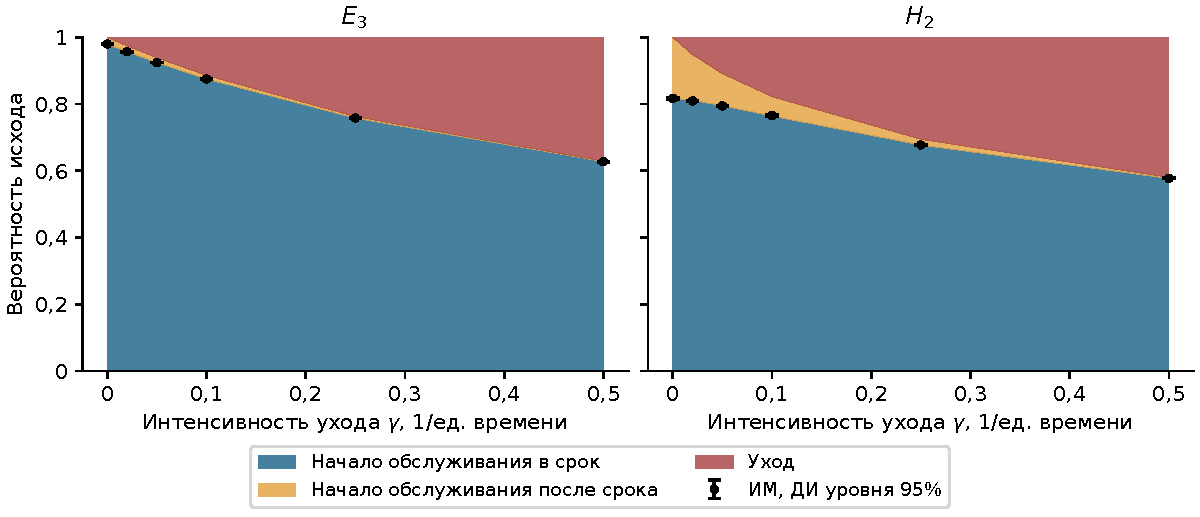
\includegraphics[width=\linewidth]{../figures/revision_outcomes.pdf}
\caption{Вероятности трёх исходов для произвольной поступившей заявки при $D=5$, $\lambda=0{,}8$, $a=2$, $b=8$. Точками отмечены оценки вероятности своевременного начала обслуживания по ИМ с доверительными интервалами уровня 95\%.}\label{fig:outcomes}
\end{figure}

\begin{figure}[htbp]\centering
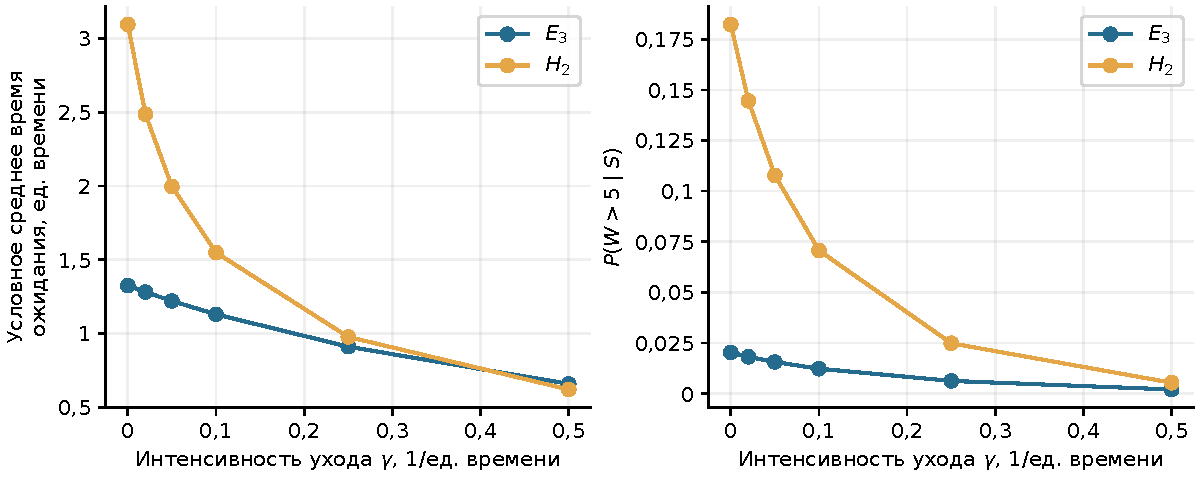
\includegraphics[width=\linewidth]{../figures/revision_conditional.pdf}
\caption{Среднее время ожидания и вероятность превышения срока при условии начала обслуживания: $D=5$, $\lambda=0{,}8$, $a=2$, $b=8$.}\label{fig:conditional}
\end{figure}

\noindent\textbf{Влияние порога и закона обслуживания.}
Порог запуска определяет соотношение времени накопления пакета и ожидания освобождения канала. На рисунке~\ref{fig:threshold} показана зависимость среднего ожидания от порога при разных нагрузках и законах обслуживания, на рисунке~\ref{fig:tails} --- значения ДФР для выбора максимального размера пакета. Выбор проводится по ДФР при заданном сроке $D$. Сопоставление ограничено исследованными сроками и не использует хвостовую асимптотику; различия вероятностей менее $10^{-7}$ считаются численно неразличимыми.

\begin{figure}[htbp]\centering
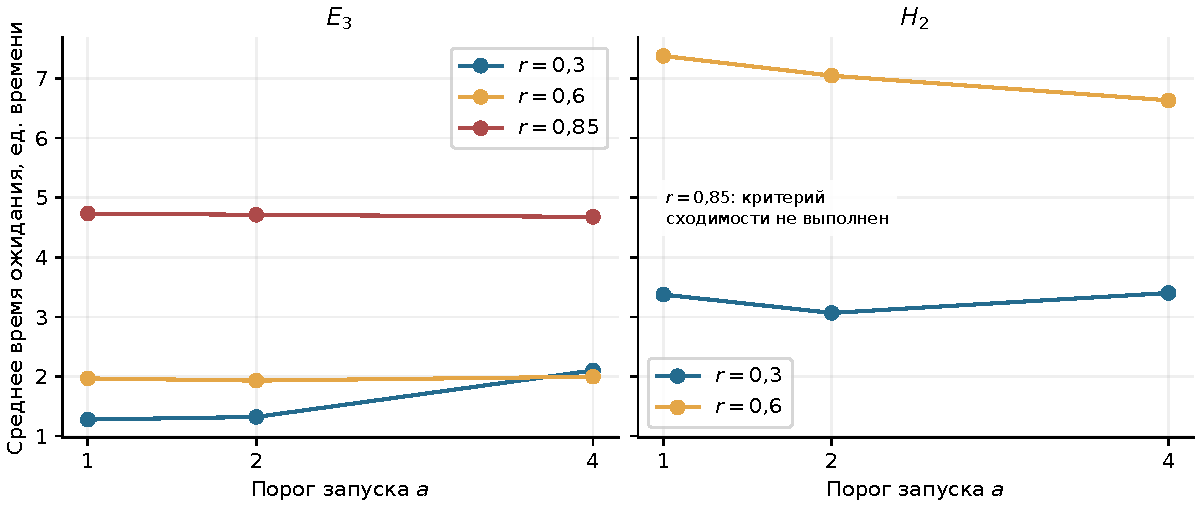
\includegraphics[width=\linewidth]{../figures/revision_threshold.pdf}
\caption{Среднее время ожидания при $b=8$, $\gamma=0$ и характеристике нагрузки $r=\lambda g(8)/8$. Для $H_2$ при $r=0{,}85$ критерий численной сходимости не выполнен.}\label{fig:threshold}
\end{figure}

\begin{figure}[htbp]\centering
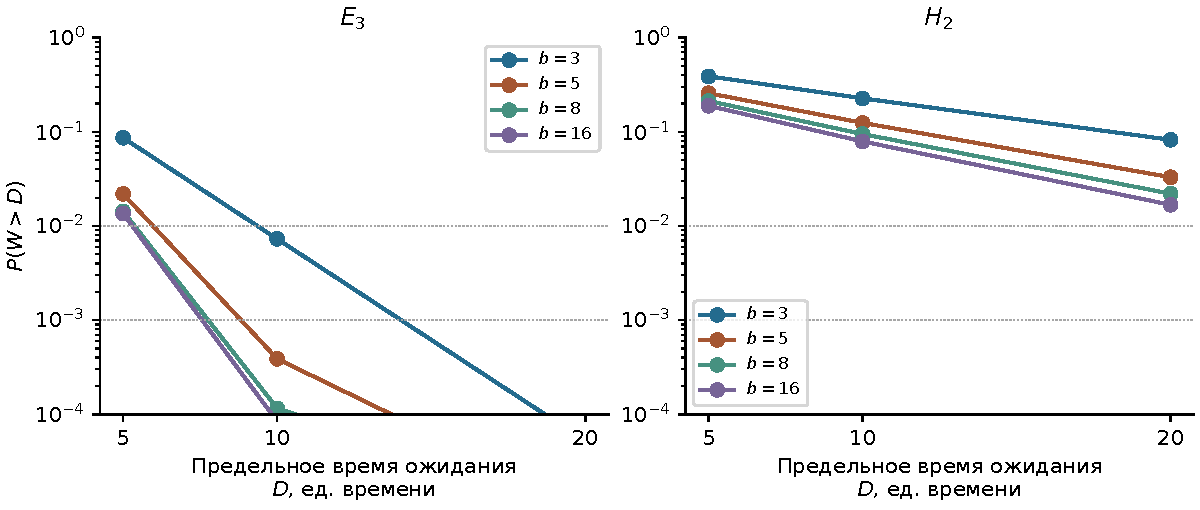
\includegraphics[width=\linewidth]{../figures/revision_tails.pdf}
\caption{Дополнительная функция распределения времени ожидания при $a=1$, $\gamma=0$, $\lambda=0{,}8$. Пунктиром обозначены уровни $10^{-2},10^{-3},10^{-4}$. Значения за нижней границей рисунка не следует считать нулевыми.}\label{fig:tails}
\end{figure}

\noindent\textbf{Аппроксимация по моментам и ошибки выбора параметров.}
Сравним два приближения условного распределения времени ожидания. В первом параметры гамма-распределения определяются по первым двум начальным моментам $m_1,m_2$ времени $W$ при условии $S$. Во втором сохраняется вероятность нулевого ожидания $z=P(W=0\mid S)$, а положительная часть распределения аппроксимируется гамма-распределением по моментам $m_n/(1-z)$; соответствующая ДФР равна $(1-z)\overline G(D)$. В таблицах эти приближения обозначены как «Гамма» и «Атом + гамма». Оба построены по одним и тем же рассчитанным моментам. Для безусловного критерия используется величина $1-p_S[1-\widehat{\overline F}_S(D)]$, где $\widehat{\overline F}_S$ --- выбранная аппроксимация, а $p_S$ сохраняет значение, рассчитанное по марковской модели. Сопоставление тем самым выделяет влияние формы аппроксимации при заданных моментах и вероятности начала обслуживания.

Для условного критерия приняты допустимые значения $\varepsilon=10^{-2},10^{-3},10^{-4}$, для безусловного --- $0{,}1;0{,}05;0{,}01$. Каждый критерий и каждое приближение проверены в 2052 сочетаниях параметров системы, срока и допуска. Ошибочным признанием допустимости назовём случай, когда по приближению требование выполнено, а по расчёту марковской модели --- нет. Ошибочное отклонение означает обратное несоответствие. Если хотя бы одно из сравниваемых значений отличается от порога не более чем на $10^{-7}$, решения считаются неразличимыми в пределах принятого численного допуска. Таких случаев в рассмотренной серии нет. Итоги приведены в таблице~\ref{tab:decisions}.

\begin{table}[htbp]\centering\small
\caption{Ошибки проверки допустимости параметров по приближённым вероятностям: 2052 проверки для каждого критерия и приближения}\label{tab:decisions}
\begin{tabular}{p{.17\linewidth}p{.21\linewidth}p{.17\linewidth}p{.15\linewidth}p{.16\linewidth}}
\hline
Критерий & Аппроксимация & Ошибочное признание допустимости & Ошибочное отклонение & Неразличимо \\
\hline
Условный & Гамма & 20 & 61 & 0 \\
Условный & Атом + гамма & 34 & 20 & 0 \\
Безусловный & Гамма & 1 & 6 & 0 \\
Безусловный & Атом + гамма & 1 & 3 & 0 \\
\hline
\end{tabular}

\end{table}

В рассмотренной серии по условному критерию учёт вероятности нулевого ожидания уменьшил общее число ошибок с 81 до 54. Число ошибочных отклонений снизилось с 61 до 20, однако число ошибочных признаний допустимости выросло с 20 до 34. Следовательно, уменьшение общего числа ошибок не обеспечивает более осторожного выбора: в этой серии недопустимые параметры чаще признавались допустимыми.

Наименьшее допустимое значение максимального размера пакета определяется как $\min\{b:\overline F_S(D)\leq\varepsilon\}$ перебором всех рассматриваемых целых значений $b$ при фиксированных остальных параметрах. Такой выбор не требует монотонности ДФР по $b$. При $E_3$-обслуживании, $a=1$, $\lambda=0{,}8$, $\gamma=0$, $D=10$ и $\varepsilon=0{,}001$ расчёт даёт $b=5$, а аппроксимация с учётом вероятности нулевого ожидания --- $b=4$. При более строгом требовании $\varepsilon=0{,}0001$ расчёт даёт $b=10$, тогда как оба приближения отклоняют все значения до 16 (таблица~\ref{tab:caps}). Следовательно, приближения могут приводить как к выбору недопустимого размера пакета, так и к исключению допустимых вариантов.

\begin{table}[htbp]\centering\small
\caption{Наименьшее значение $b\in\{2,\ldots,16\}$, удовлетворяющее условию $\overline F_S(D)\leq\varepsilon$, при $E_3$-обслуживании, $a=1$, $\lambda=0{,}8$, $\gamma=0$. Прочерк --- отсутствие допустимого значения в этом диапазоне}\label{tab:caps}
\begin{tabular}{rrrrr}
\hline
$D$ & $\varepsilon$ & Расчёт & Гамма & Атом + гамма \\
\hline
5 & 0,01 & --- & --- & --- \\
5 & 0,001 & --- & --- & --- \\
5 & 0,0001 & --- & --- & --- \\
10 & 0,01 & 3 & 3 & 3 \\
10 & 0,001 & 5 & 5 & 4 \\
10 & 0,0001 & 10 & --- & --- \\
20 & 0,01 & 3 & 3 & 3 \\
20 & 0,001 & 3 & 3 & 3 \\
20 & 0,0001 & 3 & 3 & 3 \\
\hline
\end{tabular}

\end{table}

Различие двух требований показано на рисунке~\ref{fig:feasible}: множества допустимых параметров для заявок, начавших обслуживание, и для всех поступивших заявок не совпадают. Безусловный критерий учитывает уход без обслуживания наряду с поздним началом обслуживания согласно~\eqref{eq:sla}.

\begin{figure}[htbp]\centering
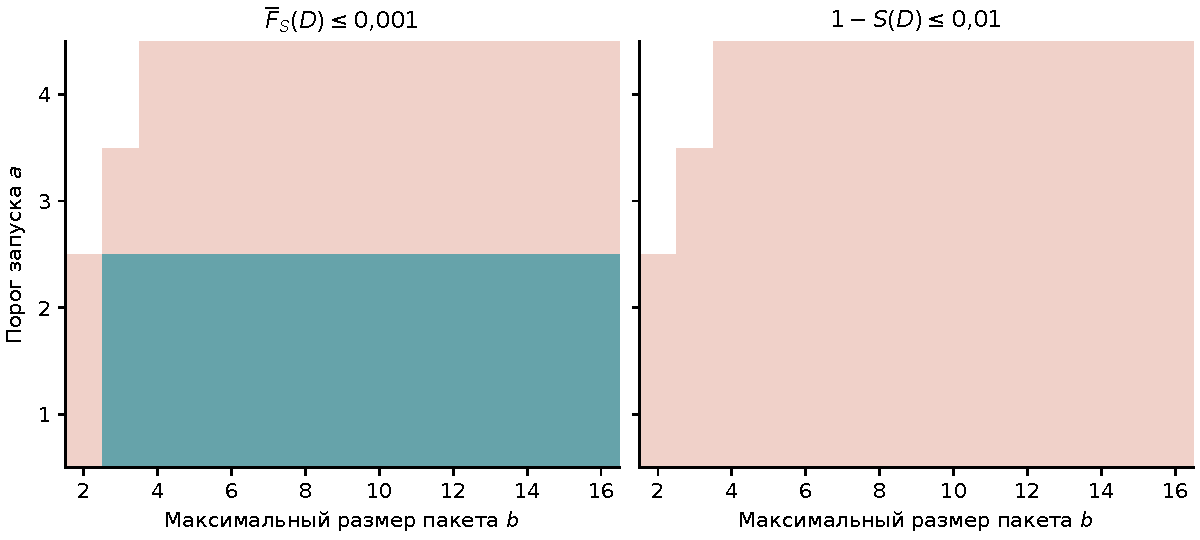
\includegraphics[width=\linewidth]{../figures/revision_feasible.pdf}
\caption{Области допустимых параметров при $E_3$-обслуживании, $\lambda=0{,}8$, $\gamma=0{,}1$, $D=10$. Синим отмечено выполнение требования, розовым --- нарушение; белые клетки соответствуют исключённым сочетаниям $a>b$. Условие $\overline F_S(D)\leq0{,}001$ не обеспечивает выполнения условия $1-S(D)\leq0{,}01$.}\label{fig:feasible}
\end{figure}

\noindent\textbf{Сопоставление с моделью Inoue.}
Влияние ограничения размера пакета можно выделить, сохранив детерминированное время обслуживания $g(i)$ и сопоставив конечные $b$ с моделью Inoue~\cite{inoue2021}. В этой работе получена оценка сверху среднего полного времени пребывания при неограниченном размере пакета (теорема~2); обозначенному там времени $W$ здесь соответствует $V$. Рассмотрены 10 вариантов: $a=1$, $\gamma=0$, $\lambda=0{,}2;0{,}8$, $b=4,8,16,32,\infty$. При конечных $b$ использовано ИМ, а при $b=\infty$ --- также расчёт по вложенной цепи Маркова. Это отдельное сопоставление по среднему времени пребывания при одинаковом законе обслуживания, а не приближение ДФР для $E_k$ или $H_2$.

\begin{table}[htbp]\centering\small
\caption{Среднее время пребывания при детерминированном обслуживании $g(i)$, $a=1$, $\gamma=0$: ИМ, расчёт по вложенной цепи и оценка сверху}\label{tab:inoue}
\begin{tabular}{rrrrr}
\hline
$\lambda$ & $b$ & ИМ: $E[V]$, 95\% ДИ & $E[V]$, расчёт & Оценка сверху \\
\hline
0,2 & 4 & [2,4404; 2,4428] & --- & --- \\
0,2 & 8 & [2,4403; 2,4427] & --- & --- \\
0,2 & $\infty$ & [2,4403; 2,4427] & 2,4422 & 2,4679 \\
0,8 & 4 & [3,2953; 3,2998] & --- & --- \\
0,8 & 8 & [3,2392; 3,2425] & --- & --- \\
0,8 & $\infty$ & [3,2391; 3,2424] & 3,2430 & 3,3532 \\
\hline
\end{tabular}

\end{table}

При $\lambda=0{,}2$ интервальные оценки среднего времени пребывания для $b=4$, $b=8$ и $b=\infty$ перекрываются. При $\lambda=0{,}8$ ограничение $b=4$ увеличивает среднее время пребывания: соответствующий ДИ целиком лежит выше интервалов для $b=8$ и $b=\infty$, которые перекрываются (таблица~\ref{tab:inoue}). Следовательно, в рассматриваемом примере влияние ограничения размера пакета зависит от интенсивности входящего потока.

При $b=\infty$ расчёт по вложенной цепи даёт среднее время пребывания $2{,}442181$ для $\lambda=0{,}2$ и $3{,}243011$ для $\lambda=0{,}8$; соответствующие оценки сверху равны $2{,}467870$ и $3{,}353239$. Во втором случае расчёт находится вне ДИ $[3{,}239147;3{,}242448]$, полученного по ИМ. Результаты относятся к двум указанным интенсивностям; применение модели с неограниченным пакетом к системе с заданным конечным $b$ требует отдельного сопоставления.

\section*{Заключение}

Построена расчётная схема для одноканальной системы с пороговым пакетным обслуживанием, простейшим входящим потоком и экспоненциальным терпением заявок. Распределение времени обслуживания фазового типа задаётся для каждого размера пакета. Цепь Маркова, описывающая ожидание меченой заявки до начала обслуживания или ухода, позволяет рассчитывать вероятности своевременного и позднего начала обслуживания, а также ухода без обслуживания. При фиксированном начальном распределении получены оценки погрешности вероятностей и ненормированных моментов, обусловленной усечением по числу заявок позади меченой.

В исследованной серии рост интенсивности ухода сопровождался сокращением среднего ожидания среди начавших обслуживание и уменьшением вероятности своевременного начала обслуживания для произвольной поступившей заявки. При выборе параметров по требованию для всех поступивших заявок поэтому необходимо учитывать оба неблагоприятных исхода: позднее начало обслуживания и уход без обслуживания.

Аппроксимация распределения ожидания по двум моментам может приводить как к ошибочному признанию допустимости параметров пакета, так и к ошибочному отклонению. В рассмотренной серии учёт вероятности нулевого ожидания уменьшил число ошибок по условному критерию с 81 до 54, но увеличил число ошибочных признаний допустимости с 20 до 34. Следовательно, такой учёт не обеспечивает односторонней погрешности решения. Расчёт вероятностей по марковской модели позволяет выбирать порог запуска и максимальный размер пакета перебором целых значений в заданном диапазоне с проверкой выбранного требования и численной сходимости.

Открытая программная реализация описанных методов доступна в библиотеке most-queue~\cite{mostqueue2026}; данные экспериментов и материалы для воспроизведения расчётов включены в электронное приложение к статье.

\printbibliography[title={Список литературы}]
\end{document}
